\documentclass[11pt]{article}
\usepackage[english]{babel}
\usepackage[utf8]{inputenc}
\usepackage{hyperref}
\usepackage{fancybox,graphicx}
\usepackage{subfig}
\usepackage{fancyhdr}
\usepackage[left=3.7cm,top=4cm,right=3.7cm,bottom=4cm]{geometry} 
\usepackage{url}
\usepackage{textcomp}
\usepackage{array}
\usepackage{enumitem}
\usepackage{caption}

\hypersetup{
	plainpages = false, pdfpagelabels,
	bookmarks,
	bookmarksopen = true,
	bookmarksnumbered = true,
	linktocpage,
	% pagebackref,
	colorlinks = true,
	linkcolor = blue,
	urlcolor  = blue,
	citecolor = green,
	anchorcolor = green,
	hyperindex = true,
	hyperfigures,
	pdfauthor={Francisco Javier P\'erez Gil},
	pdfcreator={Francisco Javier P\'erez Gil},
	pdftitle={SciFE User Guide}
}

\DeclareFontFamily{\encodingdefault}{\ttdefault}{\hyphenchar\font=`\-}
\graphicspath{{./img/}}

\lhead{}
\chead{\textsc{SciFE User Guide}}
\rhead{}
\lfoot{Fco. Javier P\'erez Gil \& Ra\'ul Moreno Gald\'on}
\cfoot{}
\rfoot{\thepage}

\renewcommand{\headrulewidth}{0.5pt} 
\renewcommand{\footrulewidth}{0.4pt} 
\pagestyle{fancy}

\renewcommand{\labelitemi}{$\bullet$}
\renewcommand{\labelitemii}{$\circ$}
\renewcommand{\labelitemiii}{$\triangleright$}

\setlength{\parindent}{0pt}
\begin{document}
\thispagestyle{empty}
\begin{titlepage}
	\begin{center}
		\textsc{\Huge SciFE User Guide}
		\vspace*{0.5in}\\
		\huge{\textsc{University of Castilla-La Mancha}}
		\vspace*{0.6in}\\
		\begin{figure}[h!]
			\centering
			\subfloat{
				
\includegraphics[scale=0.40]{logo_esii}}
			\hspace{.5cm}
			\subfloat{
				
\includegraphics[scale=0.60]{uclm.jpg}}
		\end{figure}
		\vspace{0.6in}
		\huge{\textbf{Authors:}\\Francisco Javier P\'erez Gil\\Ra\'ul Moreno Gald\'on}
	\end{center}
\end{titlepage}
\newpage
\thispagestyle{empty}
\tableofcontents
\clearpage
\thispagestyle{empty}
\listoffigures
\clearpage
\setcounter{page}{1}

\section{Introduction}
This user manual explains the user how to use the SciFE application. Information is structured in different sections, each one contains the instructions about a subject: experiment, applications, and so on.

\section{Experiments}
This section explains the user how to operate the ScifE platform to work with experiments.

\subsection{Index}
The main view of SciFE is the index, where all experiments are listed. The user can access this view clicking in ``Experiments'' link in the navbar (see Figure \ref{fig:index} in yellow colour). The index view (Figure \ref{fig:index}) shows a experiment list with a brief information of each experiment. All the experiments are shown in an accordion. Experiment information can be viewed by clicking its name in the list. Each experiment have a colour bar which changes its colour depending of the experiment status. For example, in the Figure \ref{fig:index}, the \texttt{X CESM} has a green colour bar, this is because its status is done. But for example, the \texttt{BCN CESM} show its bar in red colour, because its status has some error.\\
There are four possible colours:
\begin{itemize}
\item
\textcolor{blue}{Blue}: The experiment is in ``created'' status. This means that it is not executing or deployed anywhere. The user can modify all experiment parameters while the status is created.
\item
\textcolor{yellow}{Yellow}: The experiment is in some deployment or execution status. As the experiment is being executing somewhere, changes in its configuration will not be effective.
\item
\textcolor{green}{Green}: The experiment is in ``done'' status. The experiment has been executed successfully and results are available in the ``Overview''.
\item
\textcolor{red}{Red}: The experiment is in one of the error status. Something has failed and must be handled by the user.
\end{itemize}
\begin{figure}[htp]
	\centering
	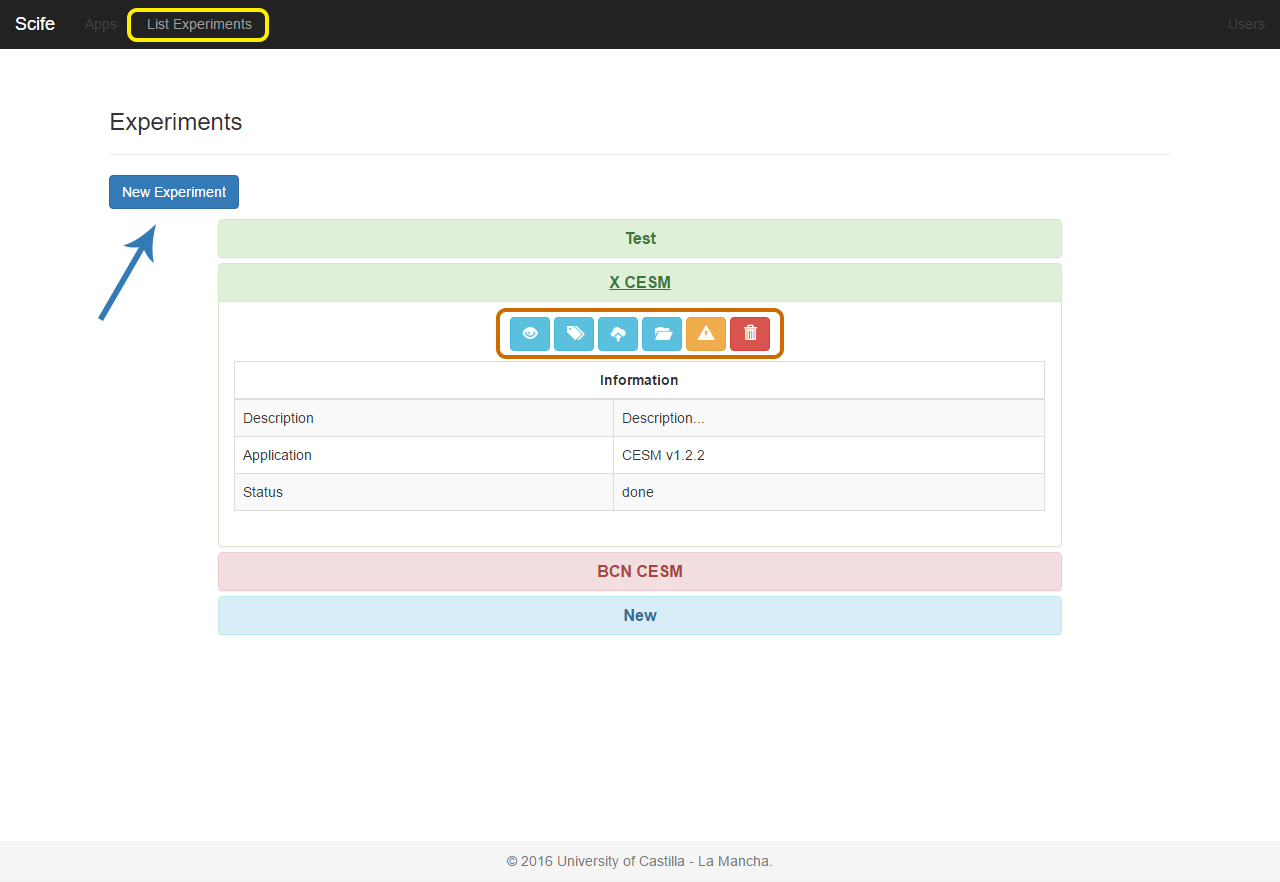
\includegraphics[width=\linewidth]{index}
	\caption{Experiment index view.}
	\label{fig:index}
\end{figure}

Some information and buttons are displayed into the selected experiment. For example, the Figure \ref{fig:index} shows the successfully executed (green) ``X CESM'' experiment with the next information:
\begin{itemize}
	\item Description: In this field the user will see the the information inserted when the experiment was created.
	\item Application: This field shows the name of the application associated with the experiment. In this case ``CESM v.1.2.2''
	\item Status: Here the user can see the specific status of the experiment, besides of the colour bar.
\end{itemize}

You can also see a series of buttons in each experiment (see Figure \ref{fig:index} marked in orange colour). This buttons allow the user browse the views of the experiment in question:
%todo Completar cada boton con la referencia a cada sección
\begin{itemize}
	\item The first button (eye open) redirect the user to the ``Overview'' view, see Section \ref{sec:overview}.
	\item The second button redirects the user to the ``Labels'' view, see Section \ref{sec:labels}.
	\item The third button opens the view that allows the user upload files to experiment, see Section \ref{sec:inputData}.
	\item The four button with an open folder redirects the user to ``Sources'' view, see Section \ref{sec:sources}.
	\item The yellow button redirects the user to the ``Logs'' view (Section \ref{sec:logs}).
	\item The red button with a trash symbol allows the user delete an experiment. When you click this button, a modal view appears to confirm the user action as can be seen in Figure \ref{fig:index-delete}. 
\end{itemize}

\begin{figure}[htp]
\centering
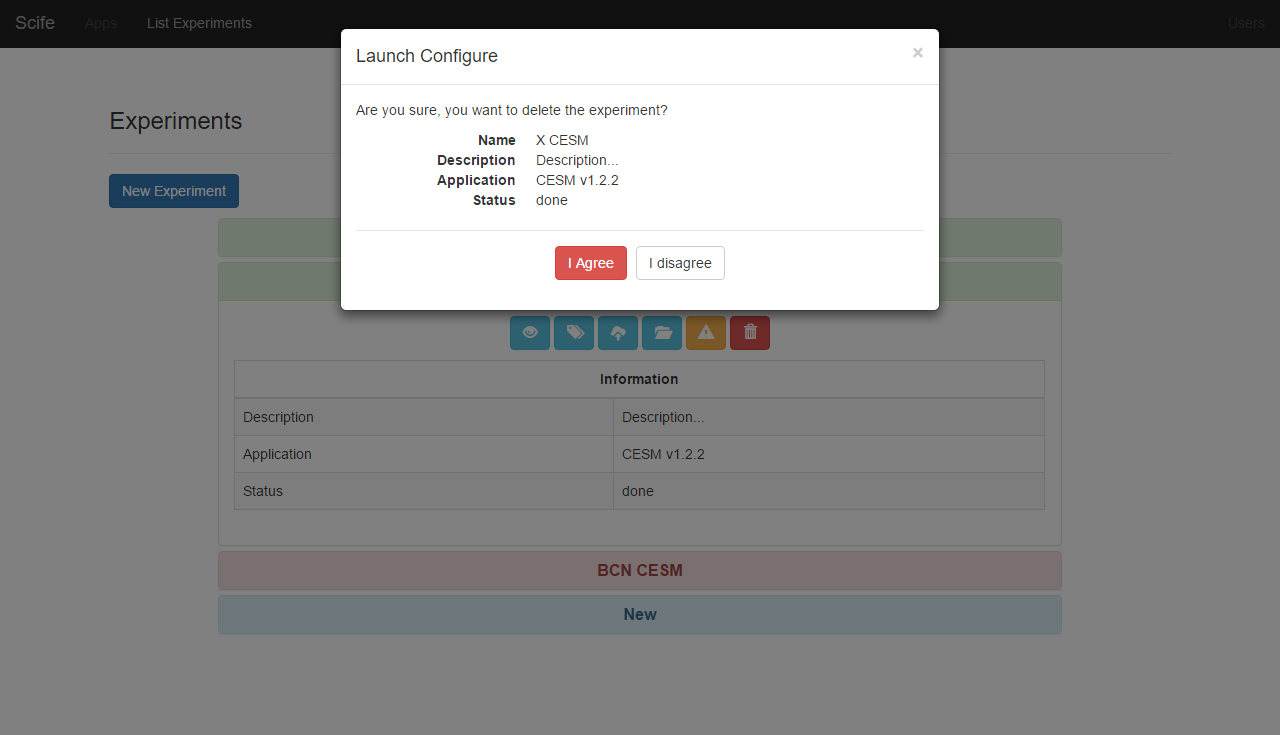
\includegraphics[width=\linewidth]{img/index-delete}
\caption{Modal view to confirm experiment deletion.}
\label{fig:index-delete}
\end{figure}

From the index view, you can create new experiments just by clicking in ``\texttt{New Experiment}'' button. After that, a new view will appear, like the one in the Figure \ref{fig:create}. You need to input some information to create the new experiment: its name, description and the application the experiment is going to use.
\begin{figure}[htp]
	\centering
	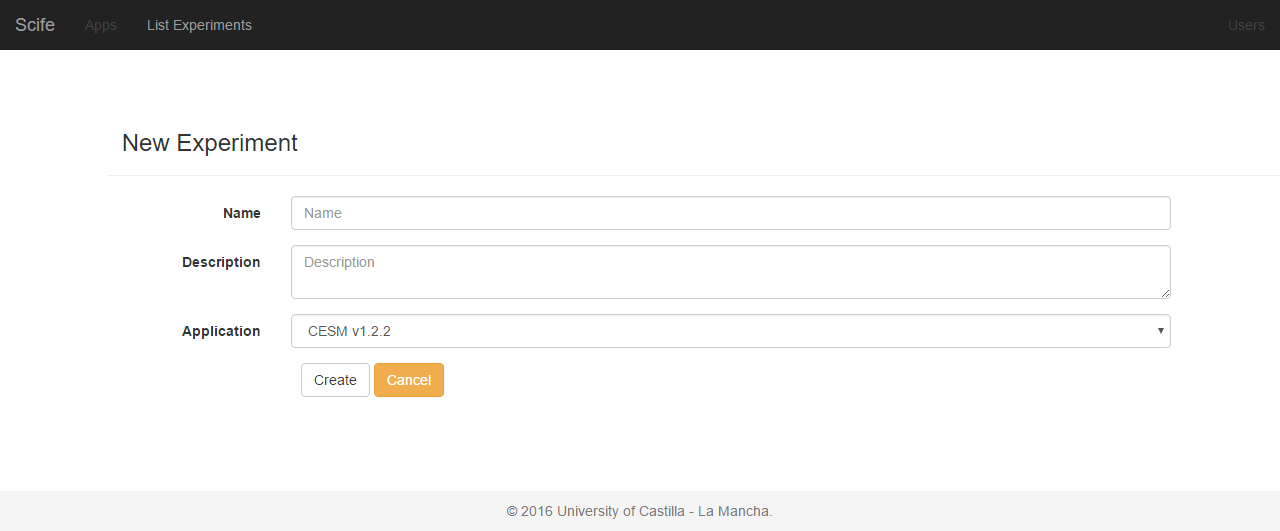
\includegraphics[width=\linewidth]{img/create}
	\caption{View with the form to create a new experiment.}
	\label{fig:create}
\end{figure}

\subsection{Overview}\label{sec:overview}
The overview is the main view of an experiment, in this page you can launch, reset, update status and delete the experiment. When the execution is successfully finished the download button is enabled to download the results of the experiment. See the Figure \ref{fig:overview-done} as example, notice the buttons in the centre of the page:
\begin{figure}[htp]
	\centering
	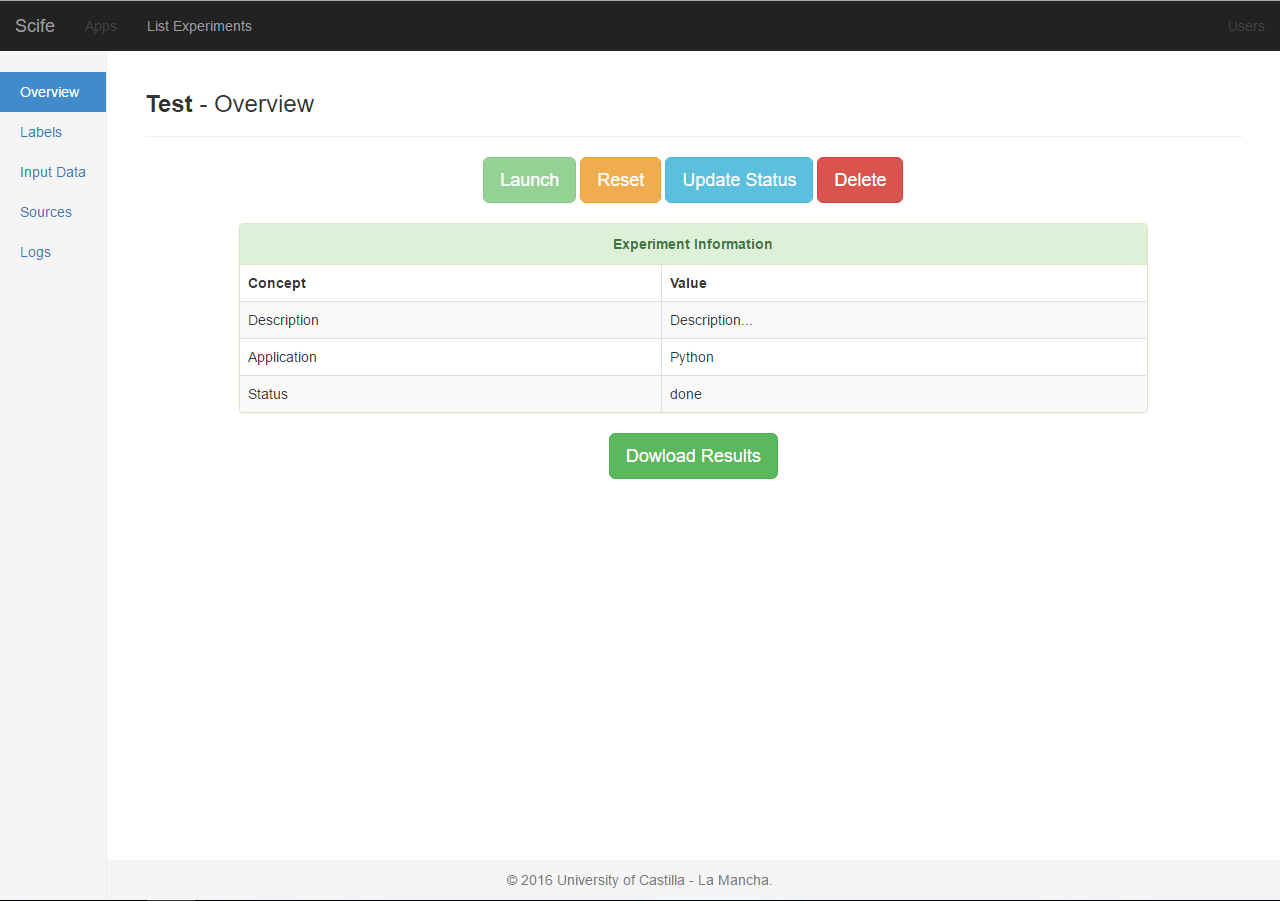
\includegraphics[width=\linewidth]{img/overview-done}
	\caption{The overview view.}
	\label{fig:overview-done}
\end{figure}

\begin{itemize}
	\item
Launch: Allow the user execute the experiment. This button is only available when the experiment status is ``created''. When you click this button, the launch form view will appear, as you can see in the Figura \ref{fig:overview-launch}. In the launch form you must select the number of nodes, the image and the size of each node where the experiment will be executed. Besides, in the bottom of the modal, you will see information about the cluster where you will execute the experiment, ``Fedora Science'' in this case. Limits for this cluster are displayed, avoiding the user to overpass them.
	\item 
Reset: Allows the user stop the experiment execution and undeploy it. ``resetting'' status will be displayed until the operations are done. This will return the experiment to the ``created'' status.
	\item
Update Status: Forces the update of the experiment information and status (launched, failed, done, etc.).
	\item
Delete: Deletes the experiment. Before do that, a confirmation form will appear. Deletion form is shown in Figure \ref{fig:overview-delete}.
\end{itemize}

\begin{figure}[htp]
	\centering
	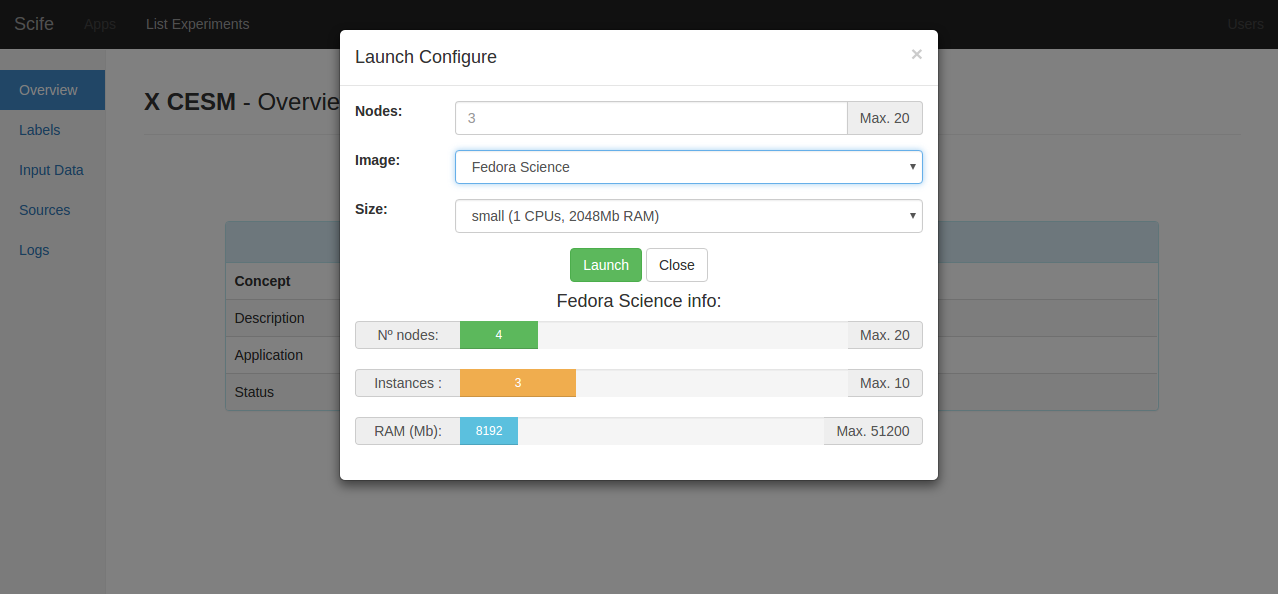
\includegraphics[width=\linewidth]{img/overview-launch}
	\caption{Launch modal view in the overview page.}
	\label{fig:overview-launch}
\end{figure}
\begin{figure}[htp]
	\centering
	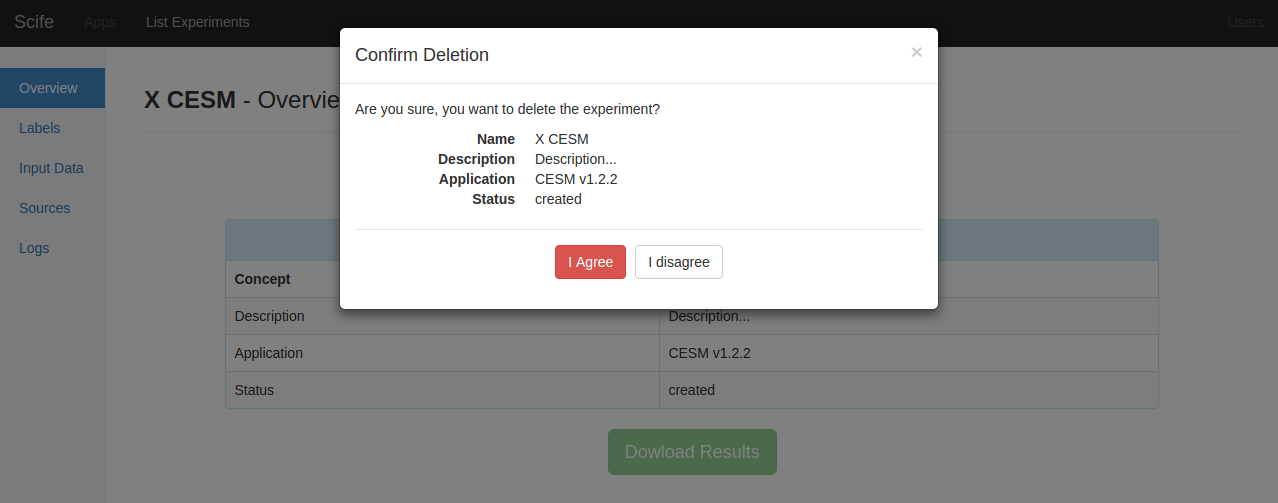
\includegraphics[width=\linewidth]{img/overview-delete}
	\caption{Confirmation of deletion modal view in the overview page.}
	\label{fig:overview-delete}
\end{figure}

\subsection{Labels}\label{sec:labels}
In this page, you can add, edit and delete the labels associated with an experiment. In the Figure \ref{fig:labels} you can see an example of the view. When you open this window, the application shows the current labels for the experiment. In Figure \ref{fig:labels} the ``\texttt{COMPSET}'' label is set to ``\texttt{X}'' and the ``\texttt{GRID\_RESOLUTION}'' label to ``\texttt{t19\_g16}'' which are the default parameters for CESM application.
\begin{figure}[htp]
	\centering
	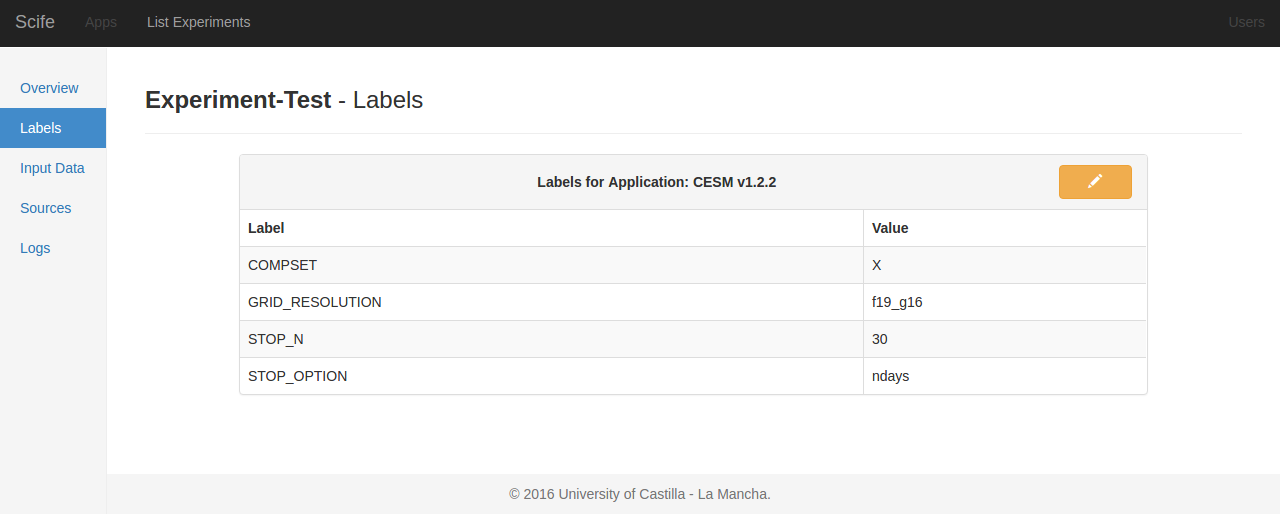
\includegraphics[width=\linewidth]{img/labels}
	\caption{Labels page of an experiment.}
	\label{fig:labels}
\end{figure}

To update (add, edit or delete) the labels, click the top-right yellow button which contains a pen icon. When you click this button a new form will be displayed as you can see in Figure \ref{fig:labels-edit}. All available labels for this experiment are shown in this form:
\begin{itemize}
	\item To add a new value to a label, just put the value you want in the label.
	\item To edit the value of a label, just modify the current value shown in the form.
	\item To delete a label, leave the field empty.
\end{itemize}

\begin{figure}[htp]
	\centering
	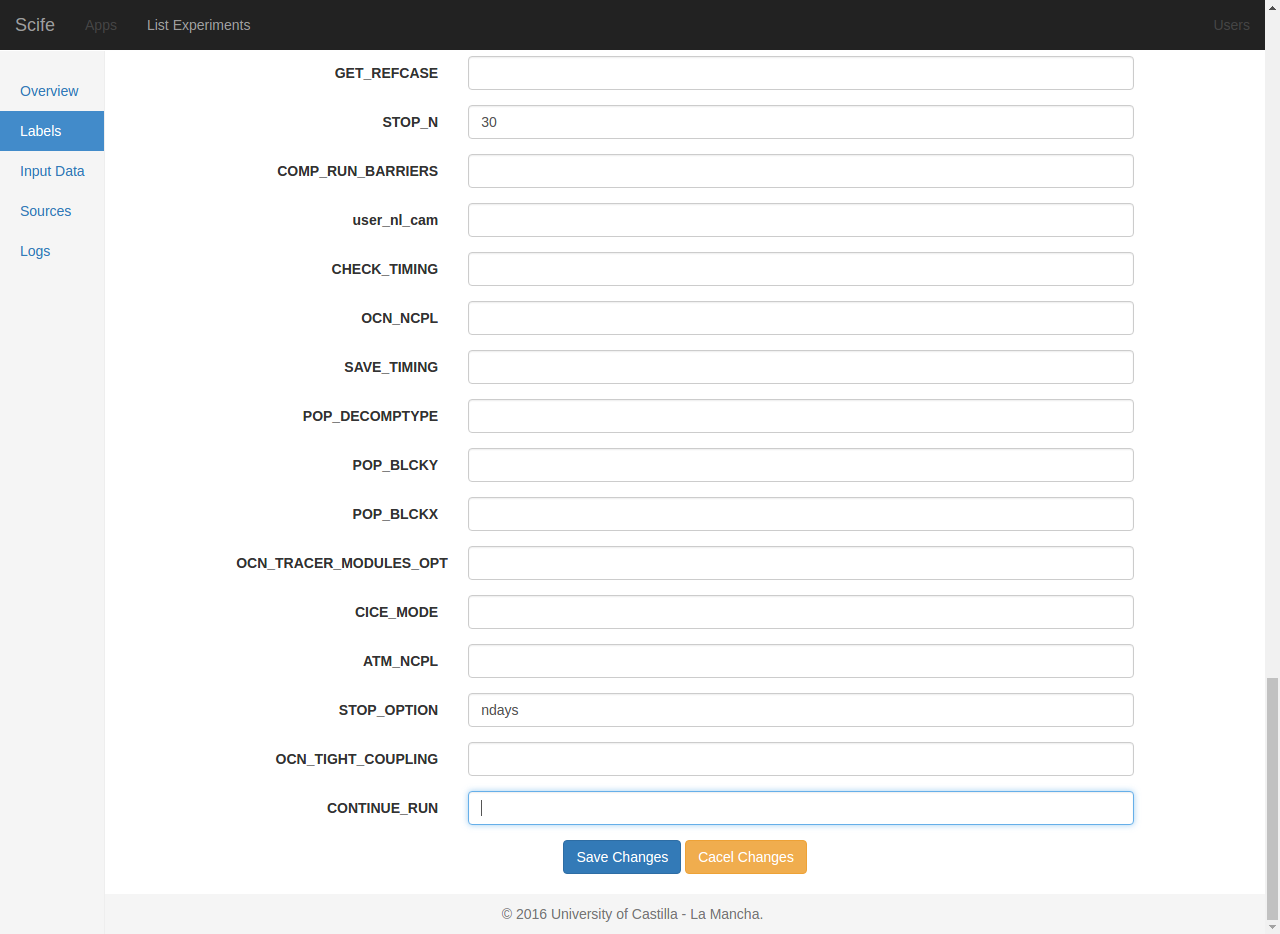
\includegraphics[width=\linewidth]{img/labels-edit}
	\caption{Form to edit the labels of an experiment page.}
	\label{fig:labels-edit}
\end{figure}

\subsection{Input data}\label{sec:inputData}
In this view, you can upload files to an experiment. The view is shown in Figure \ref{fig:input-data}, which is divided in two main parts.\\
\begin{figure}[htp]
	\centering
	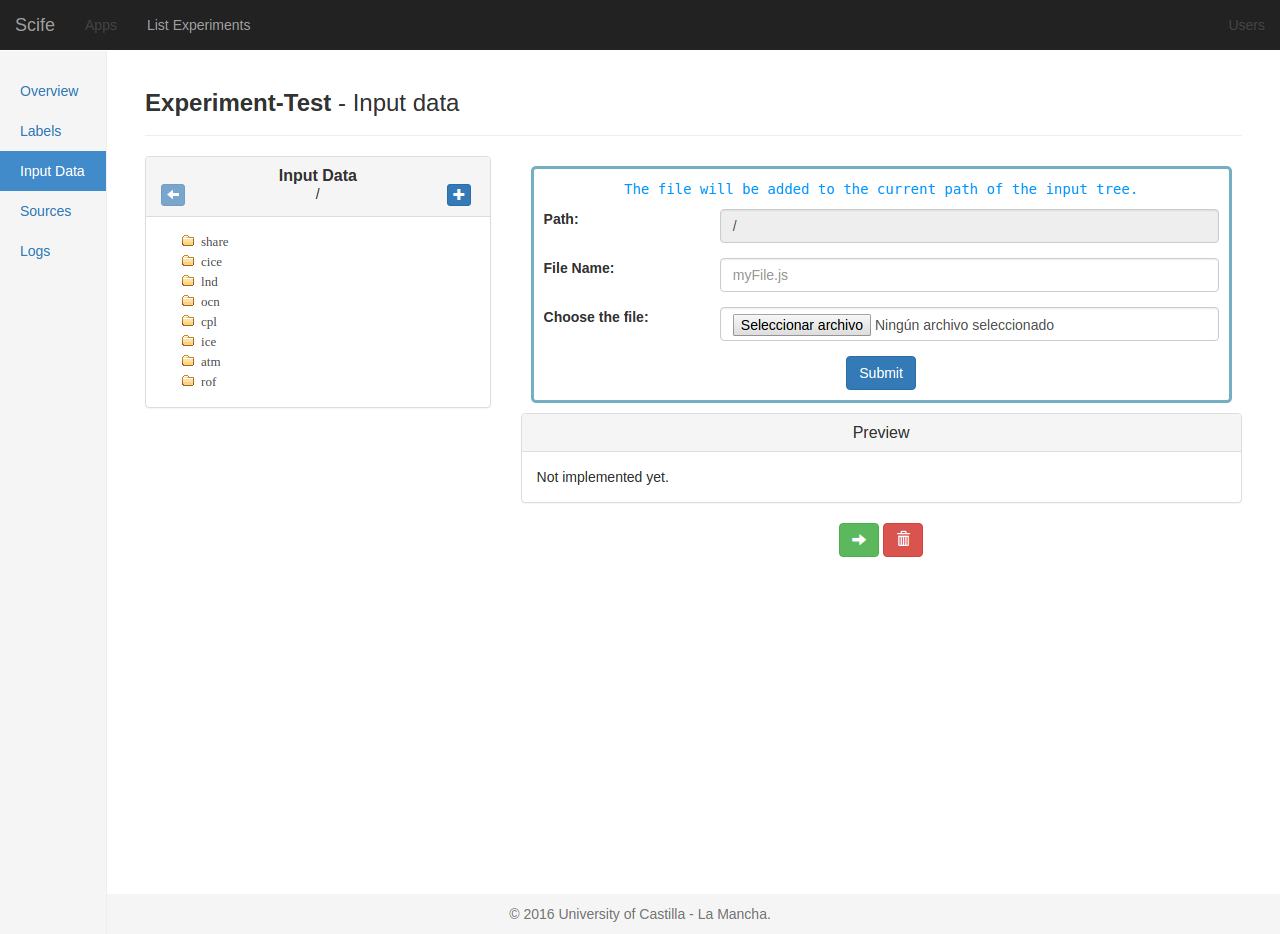
\includegraphics[width=\linewidth]{img/input-data}
	\caption{Input data view of an experiment.}
	\label{fig:input-data}
\end{figure}

In the left side, a folder tree can be seen with the files and folders you have in the platform. When a folder is clicked a new tree view appears with the contents of this folder. You can return to the parent folder with the button marked with in green colour. In the root folder ``/'', this button is disabled. To create a new folder, click in the button marked in red colour. After clicking this button, a new modal view is shown like in Figure \ref{fig:input-create-folder}. In this form the path where the folder will be created is displayed, just put the name of the new folder.
\begin{figure}[htp]
	\centering
	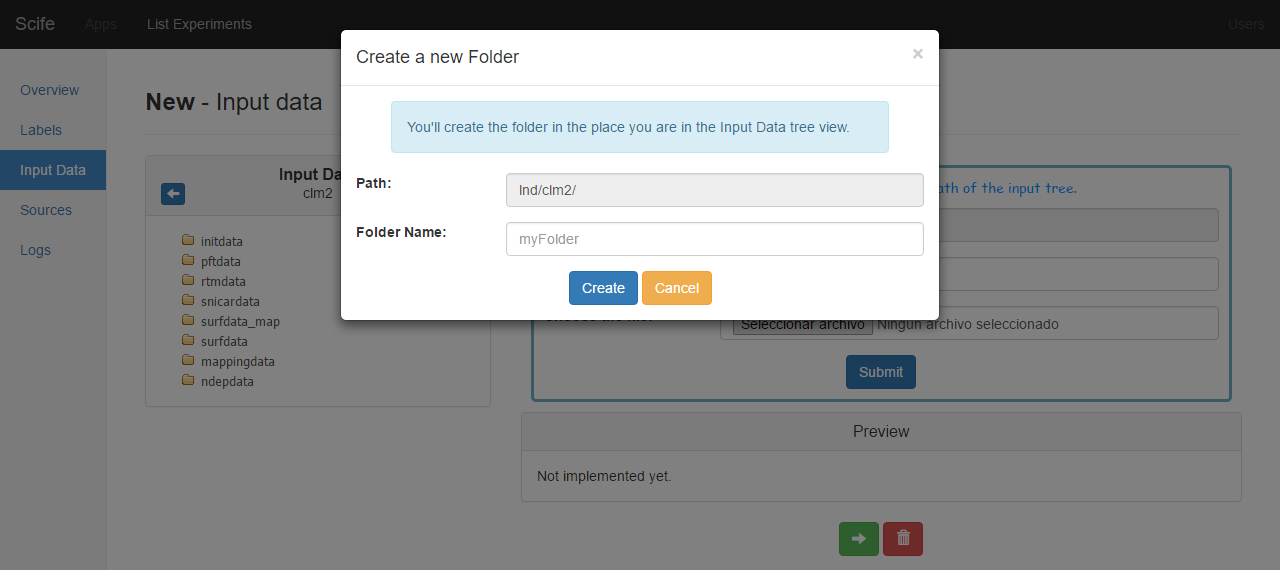
\includegraphics[width=\linewidth]{img/input-create-folder}
	\caption{Form view to create a new folder in the input data view.}
	\label{fig:input-create-folder}
\end{figure}

In the right side of Figure \ref{fig:input-data} (blue rectangle) there is a form where the user can upload a file in the current folder. Besides, the ``\texttt{Path}'' shows the path where the file will be saved.

\subsection{Sources}\label{sec:sources}
This page allows the user to edit the files of an experiment. Figure \ref{fig:sources} shows this view. In the left side, similar to input data view, you can browser the source files and folder. If you click a folder the tree view will show the contents of the selected folder, but if you click a file, the contents of the file will be shown in the code editor (right-side). To create a new folder, click the button marked with green colour and a form view will appear (Figure \ref{fig:input-create-folder}).\\
\begin{figure}[htp]
	\centering
	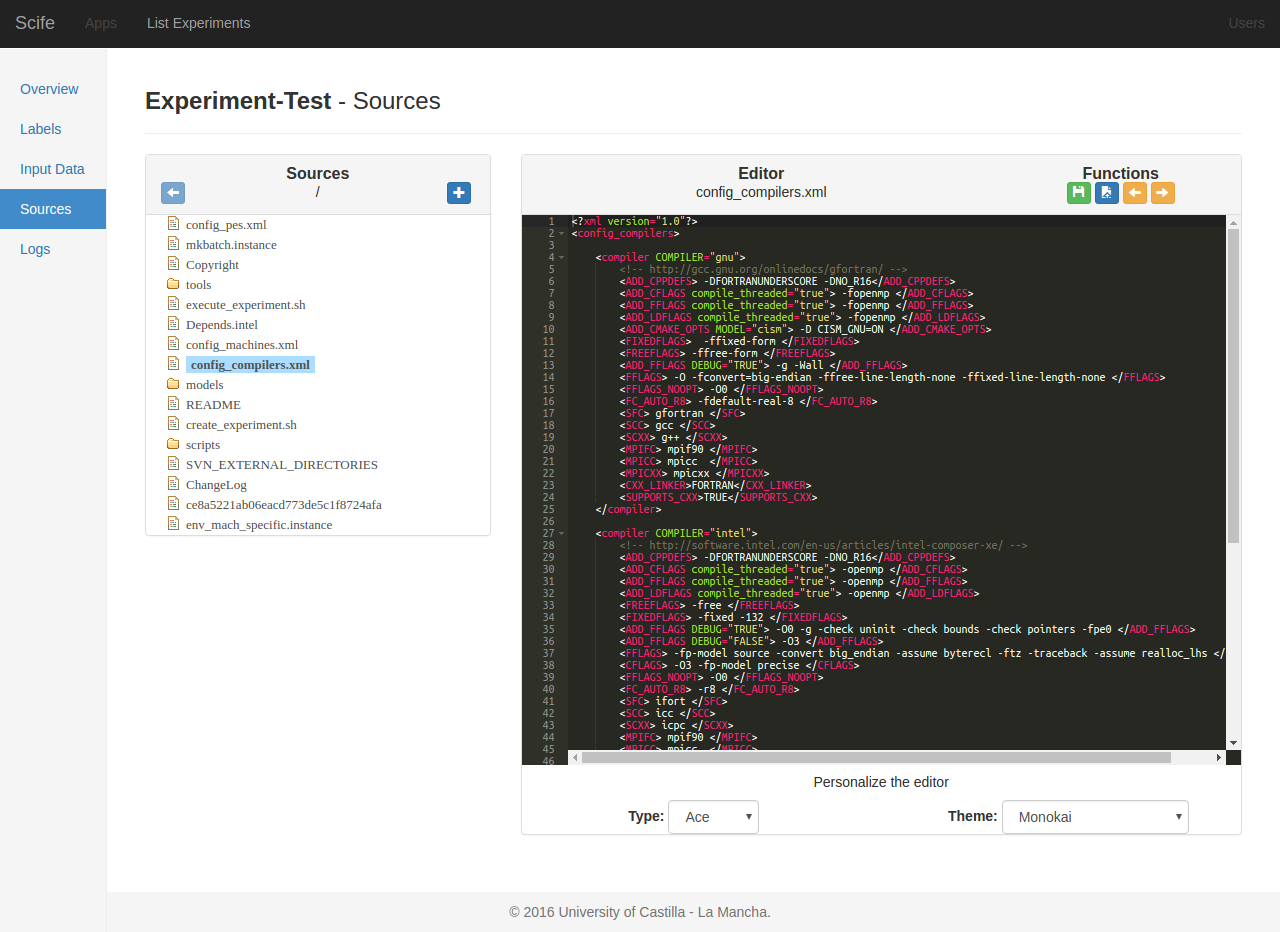
\includegraphics[width=\linewidth]{img/sources}
	\caption{Sources view of an experiment.}
	\label{fig:sources}
\end{figure}

When a file is selected, its contents appear in the code editor where them can be edited. Code editor can be customized, modifying the editor type (ace, vim or emacs) or select a theme from the long list in the bottom of the view. In the top-right side of the editor there are four buttons with the next functions:
\begin{itemize}
	\item The first green button allows the user save the changes made to the file.
	\item The second blue button allows the user create a new file with the current contents shown in the editor. After clicking this button, a form view is shown (Figure \ref{fig:sources-new-file}). Here the name of the new file must be provided. The path where the file will be created is shown too.
	\item The button with a left arrow revert/undo the changes made in the editor.
	\item The button with a right arrow remade/redo the changes previously reverted.
\end{itemize}
\begin{figure}[htp]
	\centering
	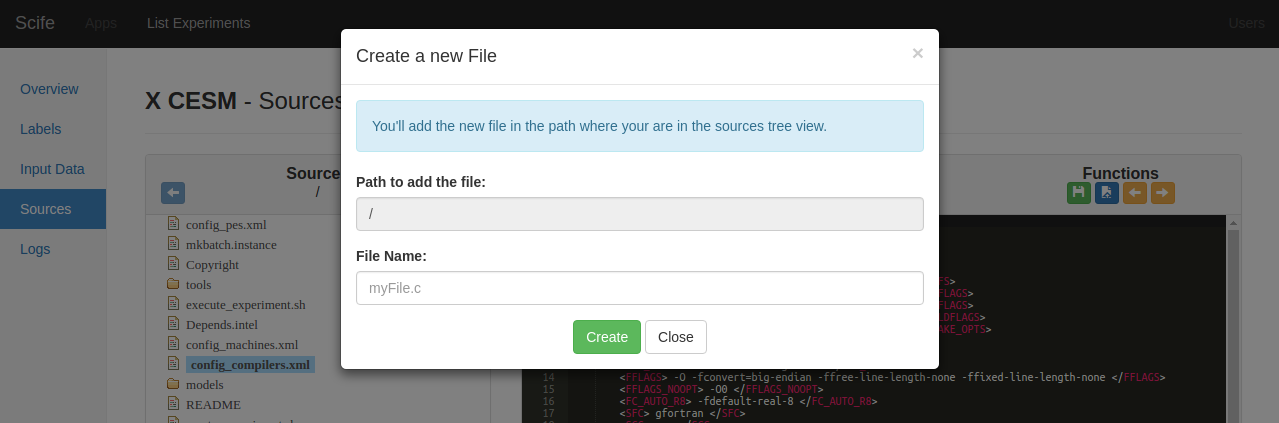
\includegraphics[width=\linewidth]{img/sources-new-file}
	\caption{Form view to create a new file in the sources view.}
	\label{fig:sources-new-file}
\end{figure}

\subsection{Logs}\label{sec:logs}
Logs generated by an executing or executed experiment are shown in this view. Figure \ref{fig:logs-listed} shows an example of this view. In this view the selection list contains a the logs filenames. If a log is selected, its contents appear in the window.
\begin{figure}[htp]
	\centering
	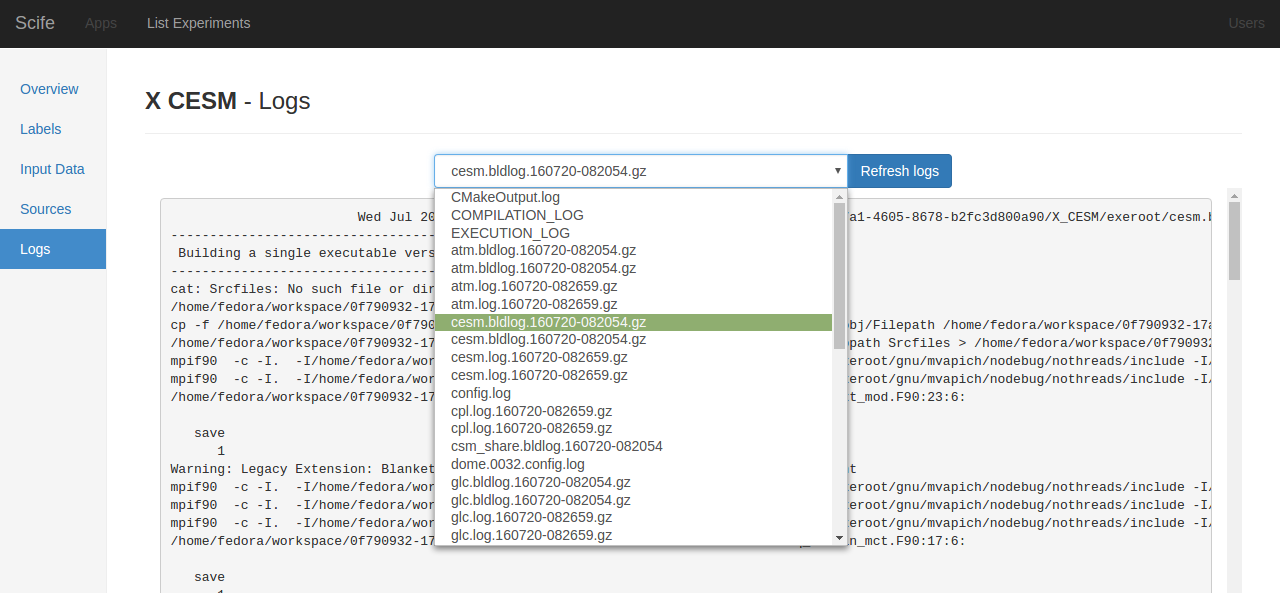
\includegraphics[width=\linewidth]{img/logs-listed}
	\caption{Sources view of an experiment.}
	\label{fig:logs-listed}
\end{figure}

\end{document}
